\section{Comparison with DCC model}
\begin{figure}
  \centering
  Model. A
  \begin{tabular}{ccc}
    \begin{minipage}{0.330\hsize}
      \centering
      $\pi^-\Sigma^+$ mode
      \includegraphics[width=4.5cm]{../pic/discussion/pimSp_A.eps}
    \end{minipage}
    
    \begin{minipage}{0.33\hsize}
      \centering
      $\pi^+\Sigma^-$ mode
      \includegraphics[width=4.5cm]{../pic/discussion/pipSm_A.eps}
    \end{minipage}
    
    \begin{minipage}{0.33\hsize}
      \centering
      $\pi^0\Sigma^-$ mode
      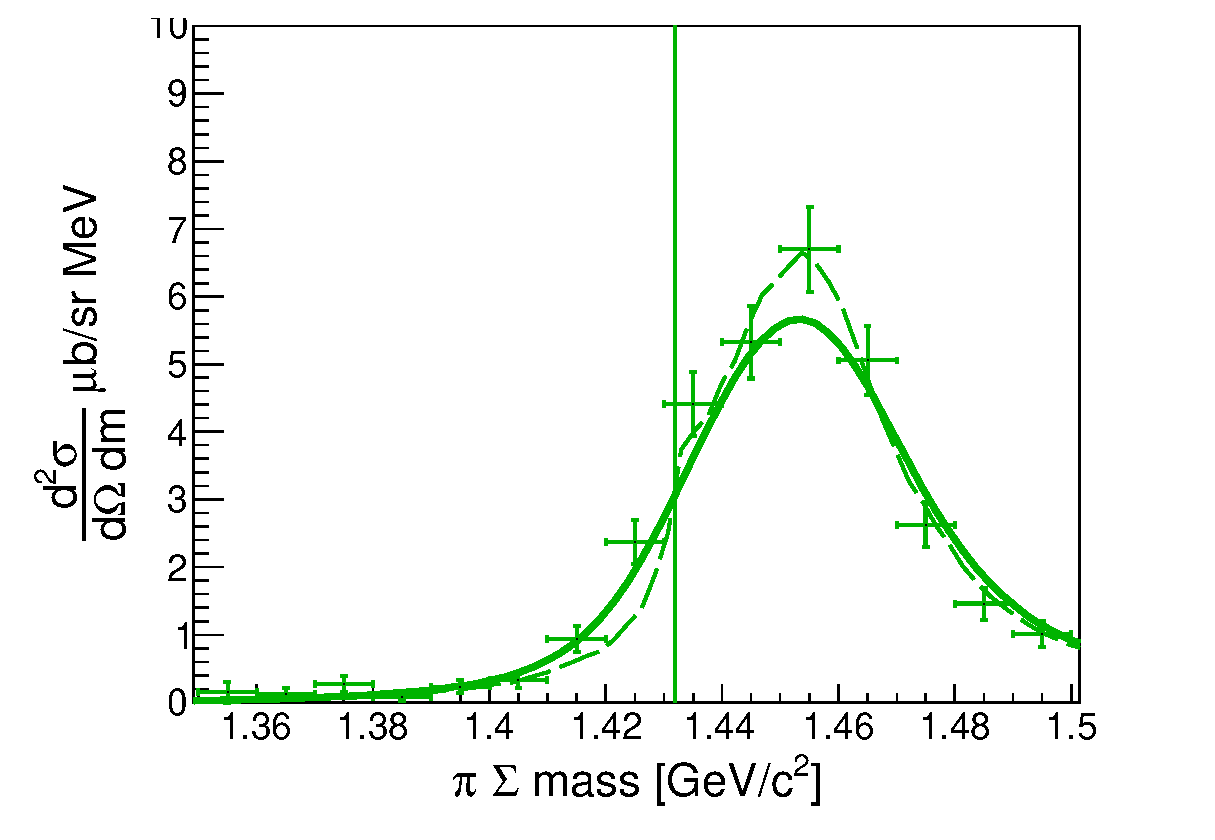
\includegraphics[width=4.5cm]{../pic/discussion/pimS0_A.eps}
    \end{minipage}
  \end{tabular}
  Model. B
  \begin{tabular}{ccc}
    \begin{minipage}{0.33\hsize}
      \centering
      $\pi^-\Sigma^+$ mode
      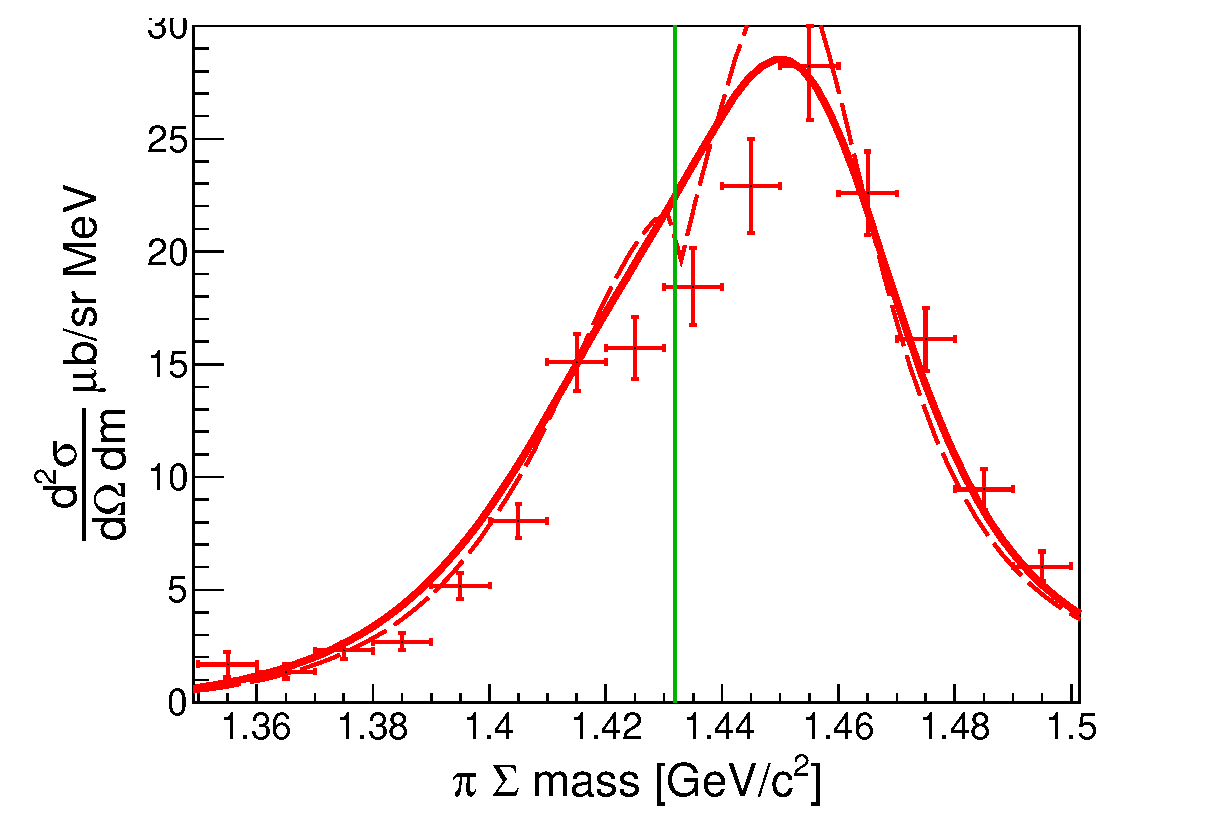
\includegraphics[width=4.5cm]{../pic/discussion/pimSp_B.eps}
    \end{minipage}
    
    \begin{minipage}{0.33\hsize}
      \centering
      $\pi^+\Sigma^-$ mode
      \includegraphics[width=4.5cm]{../pic/discussion/pipSm_B.eps}
    \end{minipage}

    \begin{minipage}{0.33\hsize}
      \centering
      $\pi^0\Sigma^-$ mode
      \includegraphics[width=4.5cm]{../pic/discussion/pimS0_B.eps}
    \end{minipage}
  \end{tabular}
  \caption{
    This figures shows obtained spectra and DCC calculation \cite{DCC2}.
    Error bar indicates obtained spectra.
    Dashed and solid line indicate theoretical calculation itself and calculation convoluted by detector resolution, respectively.
    Left, center and right figures represent \pimSp, \pipSm and \pimSz, respectively.
  }
  \label{fig:compDCC}
\end{figure}

\begin{figure}
  \centering
  \begin{tabular}{ccc}
    \begin{minipage}{0.330\hsize}
      \centering
      $I=0$\\
      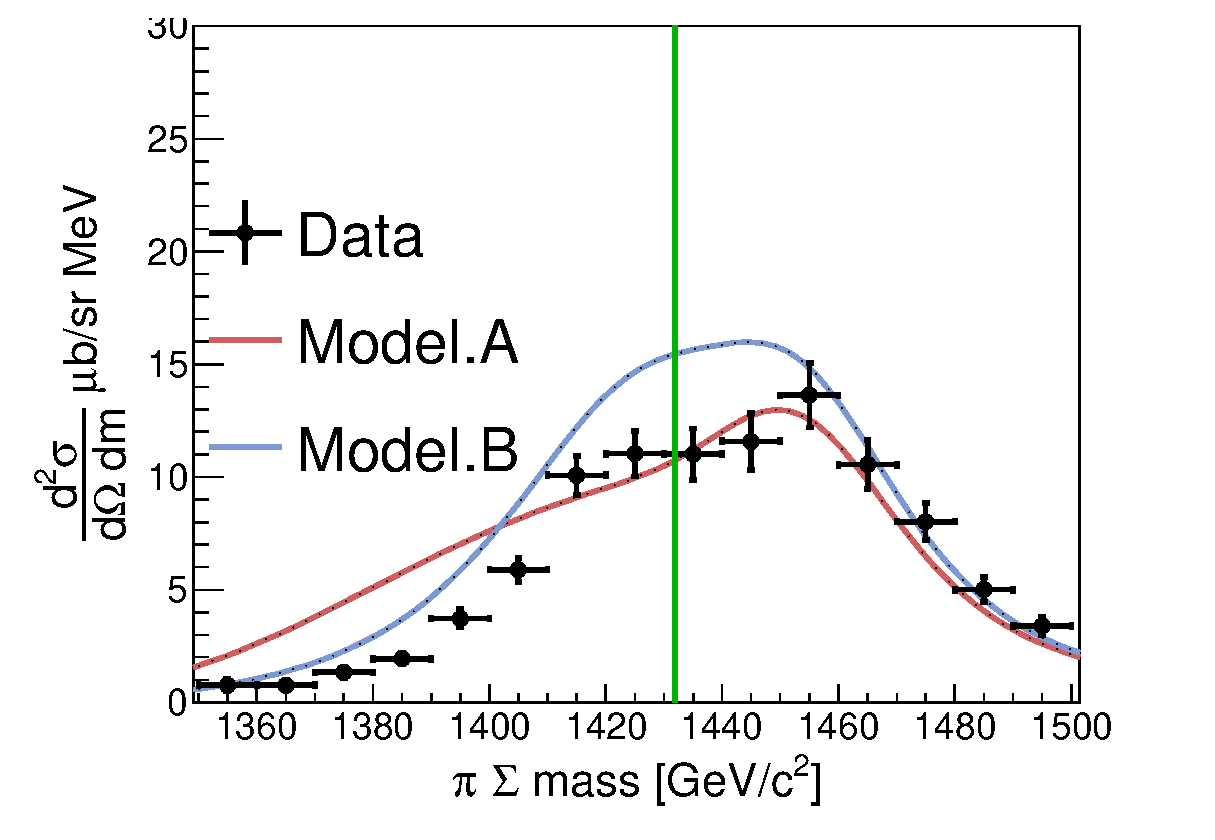
\includegraphics[width=4.5cm]{../pic/Dron/I0_comp.eps}
    \end{minipage}

    \begin{minipage}{0.33\hsize}
      \centering
      Interfer\\
      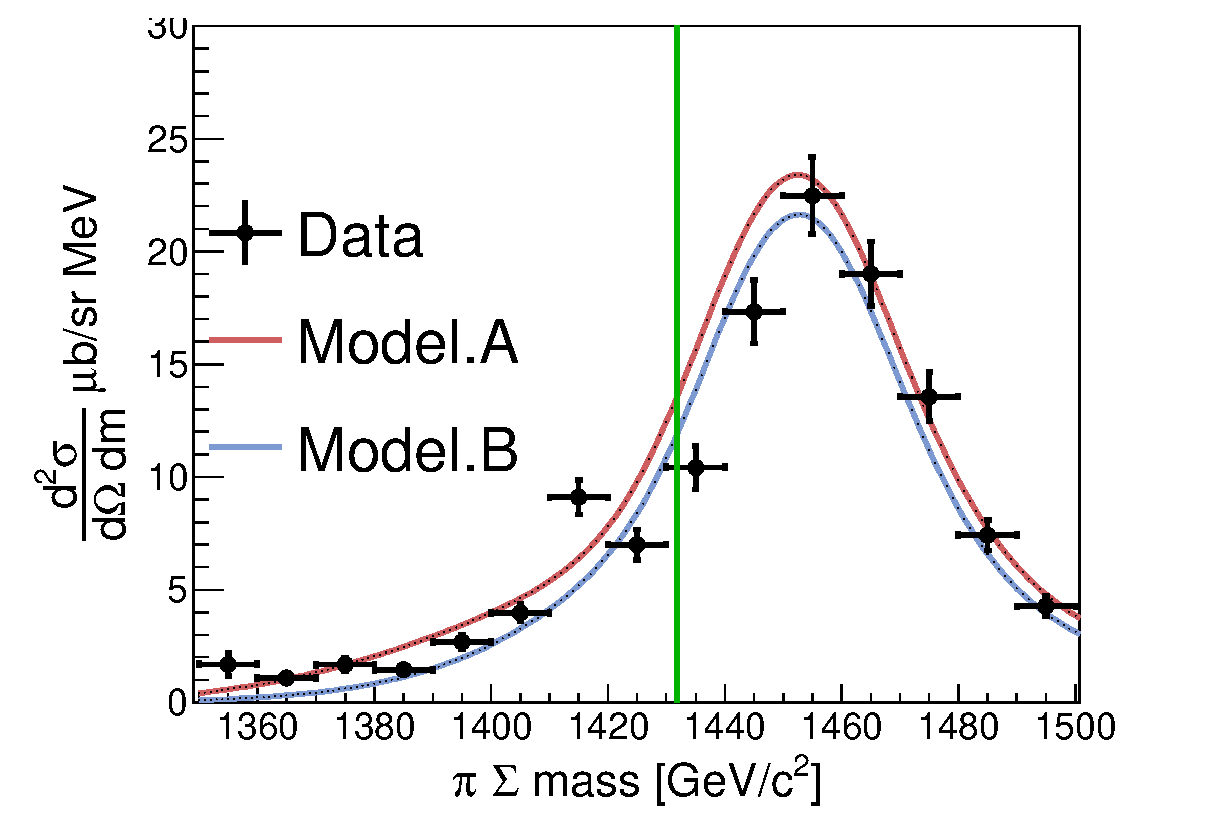
\includegraphics[width=4.5cm]{../pic/Dron/interfer_comp.eps}
    \end{minipage}

    \begin{minipage}{0.33\hsize}
      \centering
      $I=1$\\
      \includegraphics[width=4.5cm]{../pic/Dron/I1_comp.eps}
    \end{minipage}
  \end{tabular}
  \caption{
    These figures show comparison with decomposed $I=0$, $I=1$ and these interference term.
    Left, center and right represent about $I=0$, interference and $I=1$ component, respectively.
    Dark red and dark blue indicate model.A and model.B, respectively.
  }
  \label{fig:decomposed_comp}
\end{figure}

The DCC model \cite{DCC} is constructed from fitting of various $K^- p \rightarrow$ meson-baryon data from the $\bar{K}N$ threshold to $W=2.1GeV/$c as described in section,
the model can treat comprehensively scattering including strangeness in wide energy region which including high energy 1-step $K^- p \rightarrow \bar{K}N$ scattering and
$\bar{K}N \rightarrow \pi \Sigma$ scattering below the $\bar{K}N$ threshold, however the region below the threshold is extrapolation.
The theoretical calculation by the model was performed \cite{DCC2}.
We ploted into same figure as shown in Fig\ref{fig:compDCC}.
The obtained data was plotted as error bars and theoretical calculation was plotted as lines.
The dashed line indicates theoretical calculation itself and the solid line indicates them convoluted by the detector resolution which shown in Fig.\ref{fig:NC_reso}.
The overall strength of each spectra is well matched,
which means this reaction mechanism seems to consider 2-step reaction of $K^-N \rightarrow \bar{K}N$ and $\bar{K}N \rightarrow \pi\Sigma$ is dominant as described in Sec.\ref{sec:kd_reaction}.

Next, we comparison with decomposed component of $I=1$, $I=1$ and these interference term as shown in Fig.\ref{fig:decomposed_comp} to discuss about detail spectra shape.
While interference term seems to be well matched each models, there are some difference about $I=0$ and $I=1$, which is different part of each spectra depend on the model.
In the case of $I=0$ channel, model.A differ about the spectrum shape.
On the other hand, model.B seems to be better matched than model.A.
The fact is considered due to large width of higher mass region pole on model.A, so model.A has a long tail component below the $\bar{K}N$ threshold, which component can not be explain the data.
Model.B is good matched about spectrum shape, but the strength of theoretical calculation is shortage.

